\documentclass[handout]{beamer}
\definecolor{lmu@green}{rgb}{0,0.58,0.25} % use structure theme to change
% Uncomment the following for handouts.
%\documentclass[handout]{beamer}
\usepackage[utf8x]{inputenc}
\usepackage{amsmath,amsfonts,amssymb}
\setbeamertemplate{navigation symbols}{}

\usetheme{LMU}
\usecolortheme{lmu}
\useinnertheme{lmu}
\useoutertheme{lmu}

% -----------------------------------------------------------------------------
%
%\newtheorem{definition}{Definition}
\newcommand{\foot}[1]{_{\mbox{\footnotesize #1}}}
\newcommand{\head}[1]{^{\mbox{\footnotesize #1}}}
%
%
\newcommand{\ones}{\mathbb{I}}
\newcommand{\nat}{\mathbb{N}}
\newcommand{\real}{\mathbb{R}}
\newcommand{\ganz}{\mathbb{Z}}
%
%
\newcommand{\RRE}{\mbox{RRE}}
\newcommand{\nnz}[1]{\mbox{nnz}(#1)}
\newlength{\Hoehe}
\renewcommand{\vec}[1]{#1}
\newlength{\GLaenge}
\setlength{\GLaenge}{3.5cm}
%
%
\definecolor{MyGrey}{gray}{0.45}
\def\bstheta{\boldsymbol{\theta}}
\def\bsalpha{\boldsymbol{\alpha}}
\def\bsk{\boldsymbol{k}}
\def\bsx{\boldsymbol{x}}
\def\bsh{\boldsymbol{h}}
%
% Centred minipage environment
%
\newenvironment{cmpage}[1]{
\begin{center}
\begin{minipage}{#1\textwidth}}%
{\end{minipage}\end{center}}
%
%
\newcommand{\POS}{\color{blue}\item [\boldmath{$+$}]}
\newcommand{\NEG}{\color{red}\item [{\boldmath$-$}]}
\newcommand{\NTR}{\color{black}\item [$\circ$]}
\newcommand{\f}[1]{\mathfrak{#1}}
\newcommand{\old}{^{\mbox{\small \color{blue} old}}}
\newcommand{\new}{^{\mbox{\small \color{red} new}}}
\newcommand{\diag}[1]{\mbox{diag}\left(#1\right)}
%
%
\newcommand{\myBlank}{\textvisiblespace}
\newcommand{\noSpace}{\makebox[0pt]{\quad}}
%
% Old style colour commands
%
\newcommand{\CB}{\color{blue}}
\newcommand{\CR}{\color{red}}
\newcommand{\CG}{\color{green}}
\newcommand{\CC}{\color{cyan}}
%
\definecolor{myWhite}{rgb}{1.00,1.00,1.00}  % real white
\definecolor{myGrey}{rgb}{0.78,0.83,0.94}   % 'light grey blue'
\definecolor{myYellow}{rgb}{1.00,1.00,0.00} % yellow
\definecolor{myOrange}{rgb}{1.00,0.65,0.00} % orange
\definecolor{myCyan}{rgb}{0.00,1.00,1.00}   % cyan
%
% Some abbrevs for setting brief code parts
%
\newcommand{\ttA}{\mbox{\texttt{A}}}
\newcommand{\ttB}{\mbox{\texttt{B}}}
\newcommand{\ttC}{\mbox{\texttt{C}}}
\newcommand{\ttD}{\mbox{\texttt{D}}}
\newcommand{\code}[1]{\mbox{\texttt{#1}}}
\newcommand{\ccode}[1]{\cemphd{\texttt{#1}}}
%
% Commands for slides taken from 'Insides'
%
\newcommand{\rst}{\textcolor{emphcolora}{\ast}}
\newcommand{\bst}{\textcolor{emphcolorb}{\ast}}
%
%
%
\definecolor{textcolor} {rgb}{0,0,0}
\definecolor{decocolor} {rgb}{0,0,0}
\definecolor{emphcolora}{rgb}{1,0,0}              % pure red
\definecolor{emphcolorb}{rgb}{0,0,1}              % pure blue
\definecolor{emphcolorc}{cmyk}{0,1,0,0}           % pure magenta
%\definecolor{emphcolord}{cmyk}{0.64,0,0.95,0.20} % sort of green
\definecolor{emphcolord}{rgb}{0,0.4,0.12}         % same as lmu@darkgreen
\definecolor{emphcolore}{cmyk}{1,0,0,0}           % pure cyan
\definecolor{linkcolor} {rgb}{0,0,0}
%
% Commands emphasising text using color
%
\newcommand{\cempha}[1]{{\color{emphcolora}#1}}
\newcommand{\cemphb}[1]{{\color{emphcolorb}#1}}
\newcommand{\cemphc}[1]{{\color{emphcolorc}#1}}
\newcommand{\cemphd}[1]{{\color{emphcolord}#1}}
\newcommand{\cemphe}[1]{{\color{emphcolore}#1}}
\newcommand{\cemphf}[1]{{\color{decocolor}#1}}
% -----------------------------------------------------------------------------
% myColorBox
% -----------------------------------------------------------------------------
\setbeamercolor{myBoxColor}{fg=black,bg=white}
\setbeamercolor{myBoxColorHead}{fg=red,bg=white}
% \newenvironment{myColorBox}[2]{%
% \begin{beamerboxesrounded}[shadow=true,lower=myBoxColor,upper=myBoxColorHead,
% width=#1\textwidth]{#2}}%
% {\end{beamerboxesrounded}}
\newenvironment{myColorBox}[2]{%
\begin{cmpage}{#1}%
\begin{beamerboxesrounded}[shadow=true,lower=myBoxColor,upper=myBoxColorHead]%
{#2}}%
{\end{beamerboxesrounded}\end{cmpage}}
%
% -----------------------------------------------------------------------------
% Math Operators, alternate greek symbols and the like
% -----------------------------------------------------------------------------
\DeclareMathOperator{\grad}{grad}
\DeclareMathOperator{\mydiv}{div}
\DeclareMathOperator{\Grad}{grad}
\DeclareMathOperator{\Div}{div}
%\newcommand{\grad}{\mbox{grad}}
%\newcommand{\mydiv}{\mbox{div}}
\renewcommand{\rho}{\varrho}
%
% -----------------------------------------------------------------------------
% Some color defintions to be compatible with XFIG
% -----------------------------------------------------------------------------
%
\definecolor{XFIGgold}{rgb}{1.00,0.84,0.00}
\definecolor{XFIGltblue}{rgb}{0.53,0.81,1.00}
\definecolor{XFIGred}{rgb}{1.00,0.00,0.00}
% -----------------------------------------------------------------------------

\usepackage{lmodern}



% centered/centred full-screen image, no title:
% This uses the entire whole screen
\newcommand{\maxFrameImage}[1]{
\begin{frame}[plain]
\begin{changemargin}{-1cm}{-1cm}
\begin{center}
\includegraphics[width=\paperwidth,height=\paperheight,keepaspectratio]
{#1}
\end{center}
\end{changemargin}
\end{frame}
}


\newenvironment{changemargin}[2]{%
\begin{list}{}{%
\setlength{\topsep}{0pt}%
\setlength{\leftmargin}{#1}%
\setlength{\rightmargin}{#2}%
\setlength{\listparindent}{\parindent}%
\setlength{\itemindent}{\parindent}%
\setlength{\parsep}{\parskip}%
}%
\item[]}{\end{list}}





% Meta information.
\title{ObsPy: A powerful instrument for seismological data software development}
\subtitle{
38th Workshop of the International School of Geophysics \\
1$^{\text{st}}$ EPOS-ORFEUS Coordination Meeting \\
Global challenges for seismological data analysis}
\author[L. Krischer]{Lion Krischer}
\date{May 27, 2012}
\institute[LMU]{Ludwig-Maximilians-University in Munich\\ Department of Earth and Environmental Sciences\\ Geophysics}

\begin{document}

% Title page.
% Use \frame[plain]{\titlepage} for a title page without decorating elements.
\frame[plain]{\titlepage}


\begin{frame}[plain]{Python and ObsPy}

    \textbf{Goals}
    \begin{itemize}
        \item Showcase the simplicity and abilities of Python.
        \item Demonstrate why it, together with ObsPy, forms a solid foundation for seismological data software development.
    \end{itemize}

\end{frame}


%%%%%%
% PYTHON SECTION

\section{A glimpse at Python}
\frame[plain]{\tableofcontents[currentsection]}


% Short overview. The first three do not have separate slides later on.
\begin{frame}[plain]{Why use Python?}
    \begin{itemize}
        \item Open Source
        \item Cross-platform
        \item General purpose language
        \item Dynamically typed
        \item Interactive shell
        \item Readability
        \item Speed
        \item "Batteries included"
        \item Mature third party libraries
        \item Language Interoperability
    \end{itemize}
\end{frame}



\begin{frame}[fragile, plain]
    \frametitle{Readability}
    \begin{itemize}
        \item \textbf{Indentation}
            \begin{itemize}
                \item Code blocks are defined by their indentation.
                \item No explicit begin or end, and no curly braces to mark where a block starts and stops. The only delimiter is a colon (:) and the indentation of the code itself.
                \pause
                \begin{myColorBox}{0.8}{}
\begin{semiverbatim}
for i in [1, 2, 3, 4, 5]:
    if i<3:
        print i,
    else:
        print i*2,
\end{semiverbatim}
                \end{myColorBox}
Output:
                \begin{myColorBox}{0.8}{}
\begin{semiverbatim}
1 2 6 8 10
\end{semiverbatim}
                \end{myColorBox}
        \end{itemize}
        \pause
        \item \textbf{Very minimalistic clean syntax \& semantics}
            \begin{itemize}
                \item Short code = Less errors!
                \item But also faster development, quicker understanding, faster typing, faster finding errors, easier to modify ...
            \end{itemize}
        \end{itemize}
\end{frame}


\begin{frame}[fragile, plain]
    \frametitle{Readability}
    \begin{itemize}
        \item \textbf{Readable syntax}
        \pause
        \begin{enumerate}
            \item Does an element exist in a list/dict:
            \begin{myColorBox}{0.8}{}
\begin{semiverbatim}
>>> 3 \textbf{in} [1, 2, 3, 4, 5]
True
\end{semiverbatim}
            \end{myColorBox}
            \pause
            \item Does a substring exist in a string:
            \begin{myColorBox}{0.8}{}
\begin{semiverbatim}
>>> 'sub' \textbf{in} 'string'
False
\end{semiverbatim}
                \end{myColorBox}
            \pause
            \item Readable boolean values and logical operators
            \begin{myColorBox}{0.8}{}
\begin{semiverbatim}
>>> a = True
>>> \textbf{not} a
False
>>> 'sub' \textbf{not in} ['string', 'hello', 'world']
True
>>> a \textbf{or} True \textbf{and not} 1==2
True
\end{semiverbatim}
            \end{myColorBox}
        \end{enumerate}
    \end{itemize}
\end{frame}

\begin{frame}[fragile, plain]
    \frametitle{Speed}
    ''Python is extremely slow and wastes memory!''
\begin{myColorBox}{0.9}{}
\begin{semiverbatim}
xvec = range(2000000)
yvec = range(2000000)
zvec = [0.5*(x+y) for x,y in zip(xvec,yvec)]
\end{semiverbatim}
\end{myColorBox}
    \begin{itemize}
    	\item 104 MB memory usage!
	\item Runs almost 8 seconds!
    \end{itemize}
\end{frame}

\begin{frame}[fragile, plain]
    \frametitle{Speed}
    Comparison with C
\begin{myColorBox}{0.9}{}
\begin{semiverbatim}
\tiny#include <stdlib.h>

main () \{
    int *avec, *bvec;
    float *cvec;
    int i, n = 2000000;
    avec = (int*)calloc( n, sizeof(int) );
    bvec = (int*)calloc( n, sizeof(int) );
    for (i=0;i<n;i++) \{
        avec[i] = bvec[i] = i;
    \}
    cvec = (float*)calloc( n, sizeof(float) );
    for (i=0;i<n;i++) \{
        cvec[i] = (avec[i]+bvec[i])*0.5;
    \}
\}
\end{semiverbatim}
\end{myColorBox}
    \begin{itemize}
    	\item 25 MB memory usage
	\item Runs about 0.1 s (almost a hundred times faster!)
    \end{itemize}
\end{frame}

\begin{frame}[fragile, plain]{Speed}
    NumPy
\begin{myColorBox}{0.9}{}
\begin{semiverbatim}
import numpy as np

xvec = np.arange(2000000)
yvec = np.arange(2000000)
zvec = (xvec+yvec)*0.5
\end{semiverbatim}
\end{myColorBox}
    \begin{itemize}
    	\item 37 MB memory usage
	\item Runs about 0.3 s
    \end{itemize}

    \textbf{$\Rightarrow$ Choose the right tool for a job.}
    \vspace{1em}

    Using Numpy yields satisfactory performance in many cases.

\end{frame}

\begin{frame}[fragile, plain]
    \frametitle{Speed}
    \textbf{Implementation time vs. execution time}
    \pause
     \begin{itemize}
    	\item Python is designed for productivity
    	\pause
    	\item No (separate) compilation step
        \begin{itemize}
	    \item No compiler problems
	    \item No makefiles
	    \item No linker problems
	    \item Faster development cycles
        \end{itemize}	    
    	\pause
    	\item When execution speed matters:
        \begin{itemize}
    	    \item Use specialized modules
    	    \item Implement time critical parts in C/C++/Fortran/Cython
      	    \item Prototyping \& profiling
      	    \item Use specialized JIT compiler
        \end{itemize}
    \end{itemize}
\end{frame}

\begin{frame}[fragile, plain]
    \frametitle{''Batteries included''}
    \begin{itemize}
        \item Extensive standard libraries:
        \begin{itemize}
            \item \textbf{Powerful string handling}
            \item \textbf{Filesystem manipulation utitilties}
            \item Data Persistence
            \item Data Compression and Archiving
            \item Cryptographic Services
            \item \textbf{Internet Protocols and Data Handling}
            \item Structured Markup Processing Tools
            \item Development Tools
            \item Multithreading \& Multiprocessing
            \item \textbf{Regular expressions}
            \item Graphical User Interfaces with Tk
            \item ...
        \end{itemize}
    \end{itemize}
\end{frame}

\begin{frame}[fragile, plain]
    \frametitle{''Batteries included''}
    \begin{itemize}
        \item Well-documented
        \item Platform independent API, but optimized for each platform
        \item One place to look first for a proven solution
        \item Reuse instead of reinvent
    \end{itemize}
\end{frame}


\begin{frame}[plain]{Must have third party libraries/tools}
    \begin{itemize}
        \item \textbf{NumPy/SciPy} - array and matrix structures, linear algebra routines, numerical optimization, random number generation, statistics routines, differential equation modeling, Fourier transforms and signal processing, image processing, sparse and masked arrays, spatial computation, and numerous other mathematical routines
        \item \textbf{matplotlib} - 2D (and limited 3D) plotting library which produces publication quality figures via a set of functions familiar to MATLAB users
        \item \textbf{SQLAlchemy} - SQL toolkit and object-relational mapper (ORM - maps classes to the database in multiple ways), supports various databases
        \item \textbf{IPython} - Enhanced interactive shell, also provides a HTML notebook
        \item \textbf{lxml}, \textbf{PyQt}, \dots
    \end{itemize}
\end{frame}

\begin{frame}[plain]{IPython HTML Notebook}
    \begin{center}
        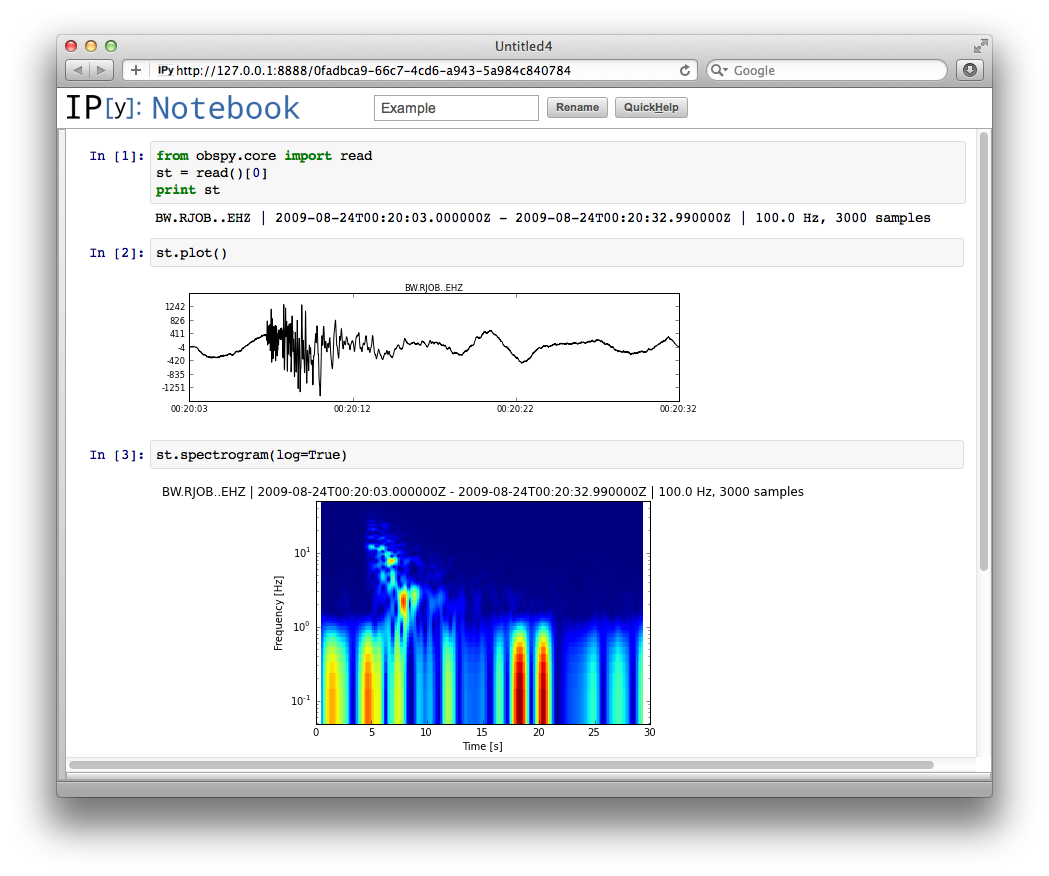
\includegraphics[height=0.95\paperheight]{images/ipy_notebook.png}
    \end{center}
\end{frame}

\begin{frame}[fragile, plain]
    \frametitle{Language Interoperability}
    Python excels at gluing other languages together: 
     \begin{itemize}
       \item \textbf{FORTRAN}: F2py - Fortran to Python interface generator (part of NumPy).
       \pause
       \item General \textbf{C} or \textbf{C++} libraries: Ctypes, Cython, or SWIG are three ways to interface them.
       \pause
       \item \textbf{R}: RPy - simple, robust Python interface to the R Programming Language. It can manage all kinds of R objects and can execute arbitrary R functions (including the graphic functions).
    \end{itemize}
\end{frame}


\section{Introducing ObsPy}
\frame[plain]{\tableofcontents[currentsection]}

\begin{frame}[plain]{What is ObsPy and what can it do}
    A Python Toolbox for seismology/seismological observatories. 

    \vspace{2em}

    The goal of the ObsPy project is to \textbf{facilitate rapid application development for seismology}. 

    \vspace{3em}

    \large
    \begin{center}
        \textbf{http://www.obspy.org}
    \end{center}
\end{frame}


\begin{frame}[plain, fragile]{What is ObsPy and what can it do}
    \begin{itemize}
        \item In development since 2008
        \item 6 core developers
        \item Many more people contribute (http://docs.obspy.org/credits.html)
        \item Thoroughly unit tested
        \item Modularized architecture
        \item Written in Python (performance critical parts are written in C)
        \item Uses well established libraries (libmseed, GSE\_UTI, \dots)
        \item Open source (LGPLv2/GPLv2) and cross platform
    \end{itemize}
\end{frame}


\begin{frame}[plain, fragile]{What is ObsPy and what can it do}
    \begin{itemize}
        \item \textbf{Read and write waveform data in various formats} (MiniSEED, SAC, GSE, SEG Y, \dots) with a unified interface.
        \item \textbf{Database and webservice access clients} for NERIES, IRIS DMC, ArcLink, SeisHub and Earthworm.
        \item \textbf{Many seismological signal processing routines} like filters, trigger, instrument correction, array analysis, beamforming, \dots
        \item \textbf{Support for inventory data} (SEED, XSEED, RESP and planned StationXML support)
        \item \textbf{Experimental event data handling} (currently only QuakeML)
        \item Waveform, spectrogram and beachball plotting, data availability (obspy-scan), \dots
    \end{itemize}
    \begin{center}
        +
    \end{center}

    \begin{center}
        \textbf{The full power and flexibility of Python.}
    \end{center}
    
\end{frame}

\begin{frame}[plain, fragile]{}
    \LARGE
    \begin{center}
        ``Live'' demonstration
    \end{center}

\end{frame}

\maxFrameImage{./images/reading_1.png}
\maxFrameImage{./images/reading_2.png}
\maxFrameImage{./images/reading_3.png}
\maxFrameImage{./images/reading_4.png}
\maxFrameImage{./images/reading_5.png}
\maxFrameImage{./images/reading_6.png}
\maxFrameImage{./images/reading_7.png}
\maxFrameImage{./images/reading_8.png}
\maxFrameImage{./images/reading_9.png}
\maxFrameImage{./images/reading_10.png}


\begin{frame}[plain]{}
    \LARGE
    \begin{center}
        Now do the same for 1000 files
    \end{center}

\end{frame}


\maxFrameImage{./images/reading_11.png}
\maxFrameImage{./images/reading_12.png}
\maxFrameImage{./images/reading_13.png}




\begin{frame}[plain]{Simple example - Reading a waveform file}
\begin{myColorBox}{0.95}{}
\begin{semiverbatim}
>>> from obspy.core import read

>>> st = read("waveform.mseed")

>>> print st

1 Trace(s) in Stream:

BW.FURT..EHZ | 2010-01-04\dots | 200.0 Hz, 7204234 samples

\end{semiverbatim}
\end{myColorBox}
\begin{itemize}
    \item Automatic file format detection.
    \item Always results in a Stream object.
    \item Raw data available as a numpy.ndarray.
\end{itemize}
\begin{myColorBox}{0.95}{}
\begin{semiverbatim}
>>> st[0].data

array([-426, -400, \dots , -489, -339], dtype=int32)
\end{semiverbatim}
\end{myColorBox}
\end{frame}

\begin{frame}[plain]{Simple example - The resulting Stream object}
 \begin{itemize}
     \item A \textbf{Stream} object is a collection of \textbf{Trace} objects
     \item A \textbf{Trace} object is a single, continuous waveform data block
     \item Working with them is easy:
         \begin{itemize}
             \item \textbf{st.filter()} - Filter all attached traces.
             \item \textbf{st.trim()} - Cut all traces.
             \item \textbf{st.resample() / st.decimate()} - Change the sampling rate.
             \item \textbf{st.trigger()} - Run triggering algorithms.
             \item \textbf{st.plot() / st.spectrogram()} - Visualize the data.
             \item \textbf{st.simulate(), st.merge(), st.normalize(), st.detrend(), \dots}
         \end{itemize}
     \item A \textbf{Stream} object can also be exported to many formats making ObsPy a good tool for converting between different file formats.
\begin{myColorBox}{0.8}{}
\begin{semiverbatim}
>>> st.write("output\_file.sac", format="SAC")
\end{semiverbatim}
\end{myColorBox}
\end{itemize}

\end{frame}


\begin{frame}[plain]{Handling time - The UTCDateTime class}
    \begin{itemize}
        \item All absolute time values are consistently handled with this class.
        \item No ambiguities, e.g. timezones, leap seconds, \dots
        \item Based on a high precision POSIX timestamp
        \item Easy usage:
\begin{myColorBox}{0.8}{}
\begin{semiverbatim}
>>> from obspy.core import UTCDateTime

>>> time = UTCDateTime(2011, 11, 11)

>>> one\_hour\_later = time + 3600

\end{semiverbatim}
\end{myColorBox}
    \end{itemize}

\end{frame}

\begin{frame}[plain]{Clients - Getting waveform data from the web}
    \textbf{ObsPy} has clients for \textbf{NERIES}, \textbf{IRIS}, \textbf{ArcLink}, \textbf{SeisHub} and \textbf{Earthworm}.

\begin{myColorBox}{0.95}{}
\begin{semiverbatim}
>>> from obspy.neries import Client

>>> from obspy.core import UTCDateTime

>>> client = Client(user="test@obspy.org")

>>> dt = UTCDateTime("2009-08-20 04:03:12")

>>> st = client.getWaveform("BW", "RJOB", "", "EH*", \

~ ~ ~ ~ ~ ~ ~ ~ ~ ~ ~ ~ ~ ~ dt - 3, dt + 15)
\end{semiverbatim}
\end{myColorBox}
\begin{itemize}
    \item Similar interfaces for the other clients.
    \item The returned Stream object is already known.
    \item Therefore it does not matter if the source of the data is the internet or a local file.
\end{itemize}
\end{frame}


\begin{frame}[plain]{Clients - Retrieving other data}
    The webservices are not limited to retrieving waveform data. Depending on the client module used, the available data includes:
    \vspace{2em}
    \begin{itemize}
        \item Event data (soon to be integrated in the new Event class).
        \item Inventory and response data.
        \item Availability information.
        \item \dots
    \end{itemize}
\end{frame}


\begin{frame}[fragile, plain]{Inventory Data}
    \begin{itemize}
        \item Can currently read/write/convert between SEED and XML-SEED.
        \item RESP file support.
        \item StationXML support is planned.
    \end{itemize}


\footnotesize
\begin{myColorBox}{0.95}{}
\begin{semiverbatim}
000001V 010009402.3121970,001,00:00:00.0000~2038,001,00:00:00.0000~
2009,037,04:32:41.0000~BayernNetz~~0110032002RJOB 000003RJOB 000008
...
\end{semiverbatim}
\end{myColorBox}

\large
\begin{center}
    $\Updownarrow$
\end{center}

\footnotesize


\begin{myColorBox}{0.95}{}
\begin{semiverbatim}
<?xml version='1.0' encoding='utf-8'?>
<xseed version="1.0">
  <volume_index_control_header>
    <volume_identifier blockette="010">
      <version_of_format>2.4</version_of_format>
      <logical_record_length>12</logical_record_length>
      <beginning_time>1970-01-01T00:00:00</beginning_time>
      <end_time>2038-01-01T00:00:00</end_time>
...
\end{semiverbatim}
\end{myColorBox}

\normalsize

\end{frame}

\begin{frame}[plain, fragile]{Events - Work in progress}
    \begin{itemize}
        \item Aims to get a unique interface independent of the data source.
        \item Currently has limited QuakeML support.
        \item In development. If you have any good ideas let us know.
    \end{itemize}
\begin{myColorBox}{0.95}{}
\begin{semiverbatim}
>>> from obspy.core.events import readEvents
>>> url = "http://www.seismicportal.eu/services/\dots"
>>> catalog = readEvents(url)
>>> print catalog
99 Event(s) in Catalog:
2012-04-11T10:43:09.400000Z |  \dots | 8.2 Mw | \dots
2012-04-11T08:38:33.000000Z |  \dots | 8.4 M  | \dots
\dots
\end{semiverbatim}
\end{myColorBox}
\end{frame}


\begin{frame}[plain]{Advanced example - Instrument correction}

\begin{myColorBox}{0.95}{}
\begin{semiverbatim}
from obspy.core import read


paz\_sts2 = \{

~ ~ ~ ~ "poles": [-0.037004 + 0.037016j, \dots

~ ~ ~ ~ "zeros": [0j, 0j],

~ ~ ~ ~ "gain": 60077000.0,

~ ~ ~ ~ "sensitivity": 2516778400.0\}


st = read()

st.simulate(paz\_remove=paz\_sts2)

\end{semiverbatim}
\end{myColorBox}
\vspace{1em}
In a real world case the response information would be read from a SEED or RESP file or retrieved from one of the webservices.


\end{frame}


\begin{frame}[plain]{What's next?}
    \begin{itemize}
            \item Getting more developers and external contributions
            \item Events
            \item StationXML
            \item More powerful correction module
            \item Suggestions? Let us know.
    \end{itemize}
\end{frame}


\begin{frame}[plain]{www.obspy.org}
    \begin{itemize}
        \item Documentation and extensive tutorial.
        \item Gallery to showcase some features.
        \item \textbf{mailing list} - subscribe for updates and discussions about the project.
        \item Source code repository and bug tracker.
        \item Automatic, daily running tests bots (http://tests.obspy.org)
        \item Get in touch!
    \end{itemize}

    \vspace{2em}

    \small
    \begin{itemize}
        \item Moritz Beyreuther et al. (2010) \textbf{ObsPy: A Python Toolbox for Seismology}, SRL, 81(3), 530-533
        \item Tobias Megies et al. (2011) \textbf{ObsPy – What can it do for data centers and observatories?} Annals Of Geophysics, 54(1), 47-58. doi:10.4401/ag-4838 
    \end{itemize}
\end{frame}


\begin{frame}[plain]{Installing ObsPy}
    \begin{itemize}
        \item \textbf{Debian/Ubuntu} - via package management (http://deb.obspy.org)
        \item \textbf{Windows} - Windows installer (automatically installs all dependencies)
        \item \textbf{OSX $\ge$ 10.6} - one-click-install application (contains all dependencies)
    \end{itemize}
    For the most recent additions and bug fixes install the developer version.
    
    \vspace{2em}

    Detailed instructions for all platforms can be found on \textbf{www.obspy.org}.
\end{frame}


\begin{frame}[plain]{Projects using ObsPy}
    \begin{itemize}
        \item NERA wavesdownloader (http://webservices.rm.ingv.it/wavesdownloader)
        \item The ADMIRE project (http://www.admire-project.eu)
        \item Antelope Python moment code (http://eqinfo.ucsd.edu/~rnewman/howtos/antelope/moment\_tensor)
        \item The new Python based Seismic Handler (http://www.seismic-handler.org)
        \item The Whisper project (http://whisper.obs.ujf-grenoble.fr)
        \item \dots
    \end{itemize}
\end{frame}


\begin{frame}[plain]{}
    \large
    \begin{center}
        \textbf{Thanks for your attention.}
    \end{center}
    \normalsize
    \vspace{1.5em}
    \begin{center}
        There are currently plans to host an ObsPy workshop in September at the ETH in Zurich. Subscribe to the \textbf{mailing list at www.obspy.org} for upcoming details.
    \end{center}
    \textbf{Credits and further reading}
    \footnotesize
    \begin{itemize}
        \item The Python Tutorial (http://docs.python.org/tutorial/)
        \item Sebastian Heimann - The Informal Python Boot Camp (http://emolch.org/pythonbootcamp.html)
        \item Hoyt Koepke - 10 Reasons Python Rocks for Research (http://www.stat.washington.edu/~hoytak/blog/whypython.html)
        \item Software Carpentry (http://software-carpentry.org/4\_0/python/)
        \item Kent S Johnson - Python Rocks! and other rants (http://kentsjohnson.com/blog/arch\_Python.html)
    \end{itemize}
\end{frame}

\maxFrameImage{./images/overview_1.png}
\maxFrameImage{./images/overview_2.png}
\maxFrameImage{./images/obspyck.png}


\end{document}
